\documentclass{report}

\input{~/latex/template/preamble.tex}
\input{~/latex/template/macros.tex}

\title{\Huge{Chapter 11.1 Notes}}
\author{\huge{Matt Warner}}
\date{\huge{}}
\pagestyle{fancy}
\fancyhf{}
\rhead{Chapter 11.2 - Series}
\lhead{\leftmark}
\cfoot{\thepage}
% \usepackage[default]{sourcecodepro}
% \usepackage[T1]{fontenc}

\usepackage{tikz}
\usepackage{pgfplots}
\pgfplotsset{compat=1.18}

\pgfpagesdeclarelayout{boxed}
{
  \edef\pgfpageoptionborder{0pt}
}
{
  \pgfpagesphysicalpageoptions
  {%
    logical pages=1,%
  }
  \pgfpageslogicalpageoptions{1}
  {
    border code=\pgfsetlinewidth{1.5pt}\pgfstroke,%
    border shrink=\pgfpageoptionborder,%
    resized width=.95\pgfphysicalwidth,%
    resized height=.95\pgfphysicalheight,%
    center=\pgfpoint{.5\pgfphysicalwidth}{.5\pgfphysicalheight}%
  }%
}

\pgfpagesuselayout{boxed}

\begin{document}
	\maketitle
	\begin{LARGE}
		\begin{center}
		\noindent \textbf{SERIES}
		\end{center}
	\end{LARGE}
\bigbreak \noindent \bigbreak \noindent \bigbreak \noindent

\begin{comment}

  ⠀⠀⠀⠀⠀⠀⠀⠀⠀⠀⠀⠀⠀⠀⠀⢀⣀⡤⠤⠤⠤⠤⠤⠤⣤⣀⣀⡀⠀⠀⠀⠀⠀⠀⠀⠀⠀⠀⠀⠀⠀⠀⠀⠀
⠀⠀⠀⠀⠀⠀⠀⠀⠀⠀⠀⠀⠀⢀⡤⠚⠁⠀⠀⠀⠀⠀⠀⠀⠀⠀⠀⠀⠉⠑⢦⡀⠀⠀⠀⠀⠀⠀⠀⠀⠀⠀⠀⠀⠀
⠀⠀⠀⠀⠀⠀⠀⠀⠀⢀⣠⠴⠚⠁⠀⠀⠀⠀⠀⠀⠀⠀⠀⠀⠀⠀⠀⠀⠀⠀⠀⠉⠒⢦⡀⠀⠀⠀⠀⠀⠀⠀⠀⠀⠀
⠀⠀⠀⠀⠀⠀⢀⡤⠖⠋⠀⠀⠀⠀⠀⠀⠀⠀⠀⠀⠀⠀⠀⠀⠀⠀⠀⠀⠀⠀⠀⠀⠀⠀⠙⢦⠀⠀⠀⠀⠀⠀⠀⠀⠀
⠀⠀⠀⠀⢀⡴⠋⠀⠀⠀⠀⠀⠀⠀⠀⠀⠀⠀⠀⠀⣀⡤⠤⠤⠶⠶⠤⠤⠤⠤⢤⣀⡀⠀⠀⠀⡇⠀⠀⠀⠀⠀⠀⠀⠀
⠀⠀⠀⠀⡾⠀⠀⠀⠀⠀⠀⠀⠀⠀⠀⢀⣠⠴⠚⠉⠁⠀⠀⠀⠀⠀⠀⠀⠀⠀⠀⠀⠉⠙⠦⣄⡇⠀⠀⠀⠀⠀⠀⠀⠀
⠀⠀⢀⡜⠁⠀⠀⠀⠀⠀⠀⠀⠀⣠⠔⠋⠀⠀⠀⠀⠀⠀⠀⠀⢠⠀⠀⠀⠀⠀⠀⠀⠀⠰⢄⣀⡹⢦⡀⠀⠀⠀⠀⠀⠀
⠀⢀⡞⠀⠀⠀⠀⠀⠀⠀⠀⣠⠞⠁⠀⠀⠀⠀⠀⠀⠀⣀⣠⠔⠋⠀⠀⠀⠀⠀⠀⠀⠀⠀⠀⡠⠖⠊⠉⠉⠐⠦⡀⠀⠀
⢀⡞⠀⠀⠀⠀⠀⠀⠀⢀⡼⠁⠀⠀⠀⠀⠀⠀⠀⠐⢋⣀⠤⠤⠤⠤⣀⠀⠀⠀⠀⠀⠀⢠⠎⠀⠀⠀⠀⠀⠀⠀⠈⢢⠀
⢸⠀⠀⠀⠀⠀⠀⠀⢀⡞⠀⠀⠀⠀⠀⠀⠀⠀⢠⠖⠉⠀⠀⠀⠀⠀⠀⠉⠢⡀⠀⠀⠀⡎⠀⠀⠀⠀⠀⠀⠀⢀⡀⠀⢣
⣼⠀⠀⠀⠀⠀⠀⠀⡼⠀⠀⠀⠀⠀⠀⠀⠀⡰⠁⠀⠀⠀⠀⠀⠀⠀⠀⠀⠀⠙⡄⠀⠀⡇⠀⠀⠀⠀⠀⠀⠀⠈⠀⠀⢸
⢿⠀⠀⠀⠀⠀⠀⢠⠇⠀⠀⠀⠀⠀⠀⠀⠀⡇⠀⠀⠀⡀⠀⠀⠀⠀⠀⠀⠀⠀⠃⠀⠀⢣⠀⠀⠀⠀⠀⠀⠀⠀⠀⠀⣸
⢸⠀⠀⠀⠀⠀⠀⣼⠀⠀⠀⠀⠀⠀⠀⠀⠀⡇⠀⠀⠘⠃⠀⠀⠀⠀⠀⠀⠀⠀⡆⠀⠀⠈⢣⡀⠀⠀⠀⠀⠀⠀⠀⡴⣧
⢸⠀⠀⠀⠀⠀⠀⡏⠀⠀⠀⠀⠀⠀⠀⠀⠀⢣⠀⠀⠀⠀⠀⠀⠀⠀⠀⠀⠀⣰⠁⠀⠀⠀⠀⣈⠓⠦⠤⠤⠤⠒⠉⠀⢸
⢸⠀⠀⠀⠀⠀⠀⡇⠀⠀⠀⠀⠀⠀⠀⠀⠀⠈⠣⣀⠀⠀⠀⠀⠀⠀⠀⣠⠔⠁⠀⠀⠀⠀⠀⠀⠑⡄⠀⠀⠀⠀⠀⠀⢸
⢸⡀⠀⠀⠀⠀⠀⡇⠀⠀⠀⠀⠀⠀⠀⠀⠀⠀⠀⠈⠙⠒⠒⠔⠒⠒⠉⠀⠀⠀⠀⠀⠀⠒⠠⠤⠚⠀⠀⠀⠀⠀⠀⠀⢸
⠀⠳⣄⠀⠀⠀⠀⢷⠀⠀⠀⡀⠀⠀⠀⠀⠀⠀⠀⠀⠀⠀⠀⠀⠀⠀⠀⠀⠀⠀⠀⠀⠀⠀⠀⠀⠀⠀⠀⠀⠀⠀⠀⠀⡼
⠀⠀⠈⠳⡀⠀⠀⠸⣆⡴⠋⠁⠀⠀⠀⠀⠀⠀⠀⠀⠀⠀⠀⠀⠀⠀⠀⠀⠀⠀⠀⠀⠀⠀⠈⡆⠀⠀⠀⠀⠀⠀⠀⢰⠇
⠀⠀⠀⠀⠳⡀⠀⠀⢻⠀⠀⠀⠀⠀⠀⠀⠀⠀⠀⠀⠀⠀⠀⠀⠀⠀⠀⠀⠀⠀⠀⠀⠀⠀⡀⢸⠀⠀⠀⠀⠀⠀⢀⠏⠀
⠀⠀⠀⠀⠀⠙⠲⢤⣼⡄⠀⠀⠀⠀⠀⠀⠀⠀⠀⠀⠀⠀⠀⠀⠀⠀⠀⠀⠀⠀⠀⠘⣆⠀⡗⠞⠀⠀⠀⠀⠀⣠⠏⠀⠀
⠀⠀⠀⠀⠀⠀⠀⠀⠀⠈⠲⢤⡤⠤⠄⠀⠀⠀⠀⠀⠀⠀⠀⠀⠀⠀⠀⠀⠀⠀⠀⠀⠈⠒⠃⠀⠀⠀⠀⢀⡴⠃⠀⠀⠀
⠀⠀⠀⠀⠀⠀⠀⠀⠀⠀⠀⠀⠙⢦⡀⠀⠀⠀⠀⠀⠀⠀⠀⠀⠀⠀⠀⠀⠀⠀⠀⠀⠀⠀⠀⠀⠀⢀⡴⠋⠀⠀⠀⠀⠀
⠀⠀⠀⠀⠀⠀⠀⠀⠀⠀⠀⠀⠀⠀⠙⠢⣄⡀⠀⠀⠀⠀⠀⠀⠀⠀⠀⠀⠀⠀⠀⠀⠀⢀⣀⡤⠒⠉⠀⠀⠀⠀⠀⠀⠀
⠀⠀⠀⠀⠀⠀⠀⠀⠀⠀⠀⠀⠀⠀⠀⠀⠀⠉⠙⠒⠦⠤⢤⣤⣤⠤⠤⠤⠤⠴⠖⠒⠛⠉⠀⠀⠀⠀⠀⠀⠀⠀⠀⠀⠀⠀

\end{comment}

\begin{LARGE}
	\noindent \textbf{Definition:}
\end{LARGE}
\bigbreak \noindent 

\begin{Large}
\noindent A \textbf{sequence} is a function whose domain is the set of positve integers. 
\end{Large}
\vspace{5mm}

% Some Graphs
\begin{mdframed}
\vspace{3mm} 

\centering
\begin{minipage}[t]{0.48\textwidth}
\centering
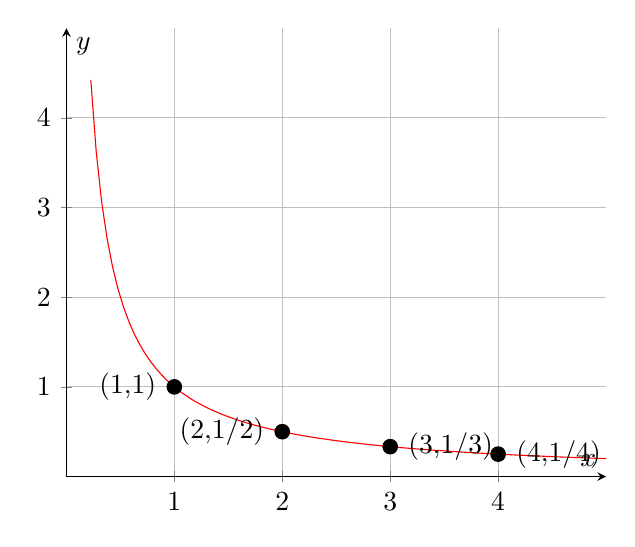
\begin{tikzpicture}
  \begin{axis}[
    restrict y to domain=0:5,
    restrict x to domain=0:5,
    samples=200,
    xmin=0,
    xmax=5,
    ymin=0,
    ymax=5,
    axis lines=middle,
    xtick={1,2,3,4},
	ytick={1,2,3,4},
    xlabel={$x$},
    ylabel={$y$},
	grid=both % This one can have some too
  ]
    \addplot [color=red] {1/x};
    \node[label={180:{(1,1)}},circle,fill,inner sep=2pt] at (axis cs:1,1) {};
    \node[label={180:{(2,1/2)}},circle,fill,inner sep=2pt] at (axis cs:2,1/2) {};
    \node[label={0:{(3,1/3)}},circle,fill,inner sep=2pt] at (axis cs:3,1/3) {};
    \node[label={0:{(4,1/4)}},circle,fill,inner sep=2pt] at (axis cs:4,1/4) {};
  \end{axis}
\end{tikzpicture}
\vspace{2mm}

$f(x)=\frac{1}{x}, x > 0$
\end{minipage}
\hfill
\begin{minipage}[t]{0.48\textwidth}
\centering
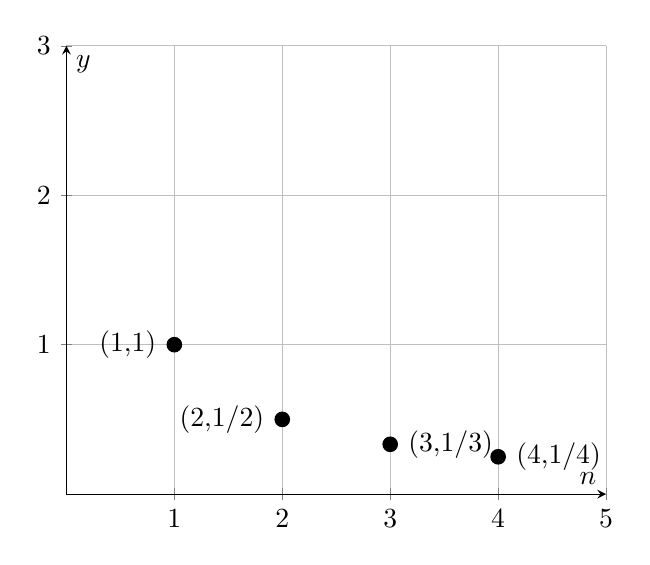
\begin{tikzpicture}
  \begin{axis}[
    restrict y to domain=0:3,
    restrict x to domain=0:5,
    samples=0,
    xmin=0,
    xmax=5,
    ymin=0,
    ymax=3,
    axis lines=middle,
    xtick={1,2,3,4,5},
	ytick={1,2,3},
    xlabel={$n$},
    ylabel={$y$},
	grid=both % looks better with gridlines
  ]
    \addplot [color=blue] {1/x};
    \node[label={180:{(1,1)}},circle,fill,inner sep=2pt] at (axis cs:1,1) {};
    \node[label={180:{(2,1/2)}},circle,fill,inner sep=2pt] at (axis cs:2,1/2) {};
    \node[label={0:{(3,1/3)}},circle,fill,inner sep=2pt] at (axis cs:3,1/3) {};
    \node[label={0:{(4,1/4)}},circle,fill,inner sep=2pt] at (axis cs:4,1/4) {};

  \end{axis}
\end{tikzpicture}
\vspace{2mm}
$f(n) = \frac{1}{n}$, n is a positive integer
\end{minipage}
\end{mdframed}
\vspace{4mm}

\nt{The graph of the left is a function
\vspace{2mm}

The graph on the right is a sequence and does not have a smooth curve, it only containts  a series of \textbf{points}
\vspace{.1mm}

A sequence uses curly braces and has subscript notation with the form $a_n$
}
\bigbreak \noindent \bigbreak \noindent 

\begin{large}
	\begin{center}
	  
	\noindent \textbf{Ex 1:} 
	Write down the first six terms of the following sequence and graph it.
	\end{center}
\end{large}
\bigbreak \noindent

 \line(1,0){450}

\begin{center}
\begin{large}
	{\LARGE{a)}} $\left\{a_n\right\}=\left\{\frac{n^{2}}{2n+1}\right\}$
\end{large}
\end{center}

\line(1,0){450}
%begin Solving -- example 1 / problem a

\begin{center}
 $a_1 = \frac{1^2}{2(1) + 2}$
 \vspace{2mm}

 $a_2 = \frac{2^2}{2(2)+1}$
 \vspace{2mm} 

 $a_3 = \frac{3^2}{2(3)+1}$
 \vspace{2mm}

 $a_4 = \frac{4^2}{2(4)+1}$
 \vspace{2mm}

 $\ldots$
\end{center}

So,
\vspace{4mm}

The first six terms of the sequence are $\frac{1}{3},\frac{4}{5}, \frac{9}{7}, \frac{16}{9}, \frac{25}{11},\frac{36}{13}$
\vspace{5mm}

\begin{center}

	\textbf{Graph of $\left(\frac{n^2}{2(n)+1}\right)$}

\begin{tikzpicture}
  \begin{axis}[
    xlabel={$n$},
    ylabel={$seq(n)$},
    only marks, % plot only the points, not a smooth curve
    mark=*,
    mark size=1.5pt, % adjust the size of the markers
	nodes near coords,
	every node near coord/.append style={font=\tiny}
    ]
    \addplot coordinates {(1, 1/3) (2, 4/5) (3, 9/7) (4, 16/9) (5, 25/11) (6, 36/13)};
  \end{axis}
\end{tikzpicture}
\end{center}
\bigbreak \noindent \bigbreak \noindent

\line(1,0){450}

\begin{center}
\begin{large}
{\LARGE{b)}} $\left\{b_n\right\}=\left\{(-1)^n \cdot 2 n\right\}$
\end{large}
\end{center}

\line(1,0){450}
% Begin Solving - example 1 / problem b

\begin{align*} b_1 & =(-1)^1(2 \cdot 1) \\ & =-2 \\ b_2 & =(-1)^2(2 \cdot 2) \\ & =4 \\ b_3 & =(-1)^3(2 \cdot 3) \\ & = -6 \end{align*}

So,
\vspace{3mm}

Continuing the sequence, the first 6 terms are $-2,4,-6,8,-10,12$
\vspace{2mm}

\begin{center}

\begin{tikzpicture}
  \begin{axis}[
    xlabel={$n$},
    ylabel={$seq(n)$},
    only marks, % plot only the points, not a smooth curve
    mark=*,
    mark size=1.5pt, % adjust the size of the markers
	nodes near coords,
	every node near coord/.append style={font=\tiny}
    ]
    \addplot coordinates {(1, -2) (2, 4) (3, -6) (4, 8) (5, -10) (6, 12)};
  \end{axis}
\end{tikzpicture}

\end{center}
\bigbreak \noindent \bigbreak \noindent

\begin{center}
 \begin{large}
	 \textbf{Ex 2:} 
	 Write down the nth term of the sequence suggested by the pattern.
 \end{large} 
\end{center}
\bigbreak \noindent

\line(1,0){450}

\begin{center}
\begin{large}
	{\LARGE{a)}} $\frac{1}{2}, \frac{1}{4}, \frac{1}{8}, \frac{1}{16}, \ldots$
\end{large}
\end{center}

\line(1,0){450}
%begin Solving - example 2 / problem a

\begin{center}
	$a_1 = \frac{1}{2^1}$
	\vspace{2mm}

	$a_{2} = \frac{1}{2^2}$
	\vspace{2mm}

	$a_{3} = \frac{1}{2^3}$
	\vspace{2mm}
\end{center}
\vspace{4mm}

So, it follows that the equation of the sequence is,
\vspace{4mm}
\begin{center}
  $\left\{a_n\right\}=\left\{\frac{1}{2^n}\right\}$
\end{center}
\bigbreak \noindent \bigbreak \noindent

\line(1,0){450}

\begin{center}
\begin{large}
	{\LARGE{b)}} $5,7,9,11, \ldots$
\end{large}
\end{center}

\line(1,0){450}
%begin solving - example 2 / problem b 

\begin{align*} b_1 & =2(1)+3 \\ & =5 \\ b_2 & =2(2)+3 \\ & =7 \\ b_3 & =2(3)+3 \\ & =9 \end{align*}
\vspace{4mm}

So, the equation of the sequence is,

$$\boxed{\left\{b_n\right\}=\{2 n+3\}}$$
\bigbreak \noindent \bigbreak \noindent

\begin{LARGE}
	\begin{center}
		\textbf{The Factorial Symbol}
	\end{center}
\end{LARGE}
\bigbreak \noindent
\begin{large}
 If $n \ge 0$ is an integer, the factorial symbol n! is defined as follows:
 \vspace{7mm}

\begin{mdframed}
	\vspace{4mm} 

 \begin{center}
  $0! = 1$
  \vspace{3mm}

	$1! = 1$
	\vspace{3mm}

	$n !=n(n-1) \cdot \ldots \cdot 2 \cdot 2 \cdot 1 \quad$ if $n \ge 2 $
 \end{center}
 \vspace{4mm}

\end{mdframed}
\end{large}
\bigbreak \noindent \bigbreak \noindent \bigbreak \noindent
\begin{large}
 \begin{center}
	 \textbf{Example 3:} 
	 Find the value of the following expressions.
 \end{center} 
\end{large}
\bigbreak \noindent

\line(1,0){450}

\begin{center}
\begin{large}
	{\LARGE{a)}} $5!$
\end{large}
\end{center}

\line(1,0){450}
% Solve here --

\begin{align*}
	5! & = 5\cdot 4\cdot 3\cdot 2\cdot 1 \\ & = 120
\end{align*}
\bigbreak \noindent \bigbreak \noindent

\line(1,0){450}

\begin{center}
\begin{large}
	{\LARGE{b)}} $6!$
\end{large}
\end{center}

\line(1,0){450}
% Solve Here --

\begin{align*}
	6! & = 6\cdot 5\cdot 4\cdot 3\cdot 2\cdot 1 \\ & =720
\end{align*}
\bigbreak \noindent \bigbreak \noindent \bigbreak \noindent

\nt{
\begin{large}
	\noindent \textbf{Write the Terms of a Sequence Defined by a Recursive Formula}
\end{large}
\vspace{3mm}

\noindent A second way of defining a sequence is to assign a value to the first (or the first few) terms(s) and specify the $nth$ term by a formula that involves one or more of the terms preceding it.
}
\bigbreak \noindent \bigbreak \noindent \bigbreak \noindent
\begin{center}
 \begin{large}
	  \textbf{Example 4:} 
	 Write down the first six terms of the following recursively defined sequence.
 \end{large} 
\end{center}
\bigbreak \noindent

\line(1,0){450}

\begin{center}
\begin{large}
$s_1=5, \quad s_n=2 \cdot s_{n-1}$
\end{large}
\end{center}

\line(1,0){450}

\begin{center}
 $s_1 = 5$
 \vspace{2mm}

$s_2 = 2 \cdot 5 = 10$
\vspace{2mm}

$s_3 = 2 \cdot 10 = 20$
\vspace{2mm}

$s_4 = 2 \cdot 20 = 40$
\vspace{2mm}

$s_5 = 2 \cdot 40 = 80$
\vspace{2mm}

$s_6 = 2 \cdot 80 = 160$
\end{center}

So,
\vspace{4mm}

The first six terms of the sequence are:
$$\boxed{5,10,20,40,80,160}$$
\newpage
\begin{LARGE}
	\begin{center}
		\textbf{Summation Noation} 
	\end{center}
\end{LARGE}
\begin{mdframed}
	\vspace{5mm}
	\begin{center}
		\begin{large}
		  
			$a_1+a_2+a_3+\cdots+a_n=\sum_{k=1}^{n} a_k$
		\end{large}
\end{center}
\vspace{5mm} 
\end{mdframed}
\bigbreak \noindent \bigbreak \noindent
\nt{The summation of $a_{k}$ from $k=1$ to $n$ is given by:
\[
  \sum_{k=1}^{n} a_k
\]
}
\bigbreak \noindent \bigbreak \noindent
\begin{center}
 \begin{large}
 \textbf{Example 5:}
 Write out each sum
 \end{large} 
\end{center}

\line(1,0){450}

\begin{center}
\begin{large}
a) $\sum_{k=1}^n \frac{k}{k+1}$
\end{large}
\end{center}

\line(1,0){450}

\begin{align*}
	\sum_{k=1}^n \frac{k}{k+1}=\frac{1}{1+1}+\frac{2}{2+1}+\frac{3}{3+1}+\cdots+\frac{n}{n+1}
\end{align*}
\bigbreak \noindent \bigbreak \noindent

\line(1,0){450}

\begin{center}
\begin{large}
(b) $\sum_{k=0}^n\left(k^2-1\right)$
\end{large}
\end{center}

\line(1,0){450}
\vspace{3mm}

\begin{center}
	$(0)^2 - 1 + (1)^2 - 1 + (2)^2 - 1 + (3)^2 - 1 + \ldots$
	\vspace{5mm}

$-1 + 0 + 3 + 8 +\ldots + (n)^2 -1$
\end{center}
\bigbreak \noindent \bigbreak \noindent
\begin{center}
 \begin{large}
	 \textbf{Example 6:} 
	 Express each sum using summation notation.
 \end{large} 
\end{center}

\line(1,0){450}

\begin{center}
\begin{large}
a) $\left(\frac{1}{1}\right)^2+\left(\frac{1}{2}\right)^2+\left(\frac{1}{3}\right)^2+\left(\frac{1}{4}\right)^2+\left(\frac{1}{5}\right)^2$
\end{large}
\end{center}

\line(1,0){450}

\begin{center}
  the numerator remains constant in each interval, while the denominator increases by a factor of one.
\end{center}

So,
\vspace{4mm}

We can conclude that the Summation notation is going to be:
$$\sum_{k=1}^5\left(\frac{1}{k}\right)^2$$ 
\bigbreak \noindent \bigbreak \noindent

\line(1,0){450}
\vspace{2mm}

\begin{center}
\begin{large}
b) $1+3+5+\cdots+2 n-1$
\end{large}
\end{center}

\line(1,0){450}
\vspace{2mm}

\begin{center}
 Given that the equation for each value of $n$ is $2n-1$, the inital value of k is one.
\end{center}

\vspace{2mm}

\begin{center}
  
 We can conclude that the Summation notation is going to be:
$$\sum_{k=1}^n 2 k-1$$
\end{center}
\bigbreak \noindent \bigbreak \noindent \bigbreak \noindent
\begin{mdframed}
  
\begin{LARGE}
 \begin{center}
	 \textbf{Properties of Sequences} 
 \end{center} 
\end{LARGE}
\vspace{4mm}

\noindent \begin{large}
  If $\left\{a_n\right\}$ and $\left\{b_n\right\}$ are two sequences and $c$ is a real number, then
\end{large}
\bigbreak \noindent 

$\begin{aligned} & \sum_{k=1}^n c=c a_1+c a_2+\cdots+c a_n=c\left(a_1+a_2+\cdots+a_n\right)=c \sum_{k=1}^n a_k \\ & \sum_{k=1}^n\left(a_k+b_k\right)=\sum_{k=1}^n a_k+\sum_{k=1}^n b_k \\ & \sum_{k=1}^n\left(a_k-b_k\right)=\sum_{k=1}^n a_k-\sum_{k=1}^n b_k \\ & \sum_{k=j+1}^n a_k=\sum_{k=1}^n a_k-\sum_{j=1}^n a_k \quad \text { where } \quad 0<j<n\end{aligned}$
\end{mdframed}
\bigbreak \noindent \bigbreak \noindent 
\begin{mdframed}
 \begin{center}
	 \textbf{Forumlas for Sums of Sequences} 
 \end{center} 
 \vspace{4mm}

$\begin{aligned} & \sum_{k=1}^n k=1+2+3+\cdots+n=\frac{n(n+1)}{2} \\ & \sum_{k=1}^n k^2=1^2+2^2+3^2+\cdots+n^2=\frac{n(n+1)(2 n+1)}{6} \\ & \sum_{k=1}^n k^3=1^3+2^3+3^3+\cdots+n^3=\left[\frac{n(n+1)}{2}\right]\end{aligned}$
\vspace{2mm}
\end{mdframed}
\bigbreak \noindent \bigbreak \noindent
\begin{large}
 \begin{center}
	 \textbf{Example 7:} 
	 Find the sum of the sequence
 \end{center} 
\end{large}

\line(1,0){450}

\begin{center}
\begin{large}
$\sum_{k=1}^{10}\left(k^2-k\right)$
\end{large}
\end{center}

\line(1,0){450}

\begin{center}
  Using the formula $\rightarrow$ $\sum_{k=1}^n k^2=1^2+2^2+3^2+\cdots+n^2=\frac{n(n+1)(2 n+1)}{6}$ for $k^2$
  \vspace{3mm}

  And $\sum_{k=1}^n k=1+2+3+\cdots+n=\frac{n(n+1)}{2}$ for $k$,
  \vspace{3mm}

  Our equation for finding the sum of the sequence is going to be:
$$
\frac{10(10+1)(2 \cdot 10+1)}{6}-\frac{10(10+1)}{2}
$$
$$ = \frac{2310}{6} - 55$$
$$ =\boxed{330}$$
\end{center}
\end{document}
